\documentclass[serif, aspectratio=169]{beamer}
%\documentclass[serif]{beamer}  % for 4:3 ratio

\usepackage[T1]{fontenc} 
\usepackage[utf8]{inputenc}
\usepackage{fourier} % see "http://faq.ktug.org/wiki/uploads/MathFonts.pdf" for other options
\usepackage{hyperref}
\usepackage{latexsym,amsmath,xcolor,multicol,booktabs,calligra}
\usepackage{graphicx,pstricks,listings,stackengine}
\usepackage{lipsum}
\usepackage{../HKUSTstyle}

%imports customs%
\usepackage{caption}    % for subfigures
\usepackage{subcaption} % for subfigures
\usepackage{ragged2e}
\usepackage{booktabs,makecell}
\usepackage{colortbl}
\usepackage{multirow}
\usepackage{cite}
\usepackage{tcolorbox}
\usepackage[sort,authoryear]{natbib}

\author{Julien Bezançon}

\title{Découverte du Traitement Automatique des Langues}
\subtitle{CM 3~: De la linguistique au TAL}

\institute{julien.bezancon@univ-lorraine.fr / \url{https://julienbez.github.io}}

\date{}

% defs
\def\cmd#1{\texttt{\color{red}\footnotesize $\backslash$#1}}
\def\env#1{\texttt{\color{blue}\footnotesize #1}}

% set colors
\definecolor{hkustyellow}{RGB}{167, 131, 55}
\definecolor{hkustblue}{RGB}{0, 56, 116}
\definecolor{hkustred}{RGB}{209, 51, 59}

\lstset{
    basicstyle=\ttfamily\small,
    keywordstyle=\bfseries\color{deepblue},
    emphstyle=\ttfamily\color{deepred},    % Custom highlighting style
    stringstyle=\color{deepgreen},
    numbers=left,
    numberstyle=\small\color{halfgray},
    rulesepcolor=\color{red!20!green!20!blue!20},
    frame=shadowbox,
}

\begin{document} %  --- --- --- --- --- --- --- --- --- --- --- --- 

\begin{frame}[noframenumbering,plain]
    \titlepage
    \vspace*{-0.6cm}
    \begin{figure}[htpb]
        \begin{center}
            \hspace{0.3cm}
            
\includegraphics[width=0.7\columnwidth]{../../../IMAGES/loria_idmc.png}
        \end{center}
    \end{figure}
\end{frame}

% \begin{frame}    
%     \tableofcontents[sectionstyle=show,
%     subsectionstyle=show/shaded/hide,
%     subsubsectionstyle=show/shaded/hide]
% \end{frame}

\section{Avant de commencer...}

\begin{exoframe}{}
    \begin{center}
        \Large
        De quoi avons-nous discuté lors du derniers cours ? \\
        Avez-vous des questions ?
    \end{center}
\end{exoframe}

\begin{frame}{Doggy bag du dernier cours}
    \begin{minipage}{0.45\columnwidth}
        \begin{block}{Tâche VS application}
            \begin{itemize}
                \item Tâche = problématique précise
                \item Application = plusieurs tâches
            \end{itemize}
        \end{block}
        \begin{block}{Tâches du TAL}
            \begin{itemize}
                \item Classification de textes
                \item Résumé automatique
                \item Analyse syntaxique
                \item Similarité
                \item ...
            \end{itemize}
        \end{block}
    \end{minipage}
    \hfill
    \begin{minipage}{0.45\columnwidth}
        \begin{figure}
            
\includegraphics[width=0.9\columnwidth]{../../../FIGURES/divers/doggybag.jpg}
        \end{figure}
    \end{minipage}
\end{frame}

\section{Introduction à la linguistique}

\begin{frame}{Rappel~: le langage selon une machine}
    \begin{block}{Ce que "voit" une machine}
        \begin{table}
            \renewcommand{\arraystretch}{1.5}  
            \raggedright
            \begin{tabular}{|l|l|}
                \hline
                Séquence (caractères) & Êl síla erin lû e-govaned vîn \\
                \hline
            \end{tabular}
        \end{table}   
    \end{block}
    \begin{block}{Ce qu'elle ne voit et/ou ne comprend pas}
        \begin{table}
            \renewcommand{\arraystretch}{1.5}  
            \raggedright
            \begin{tabular}{|l|l|}
                \hline
                Syntaxe (structure) & \fcolorbox{black}{red!20}{\fcolorbox{black}{red!20}{Êl} \fcolorbox{black}{red!20}{síla} \fcolorbox{black}{red!20}{erin}} \fcolorbox{black}{blue!20}{\fcolorbox{black}{blue!20}{lû} \fcolorbox{black}{blue!20}{e-govaned} \fcolorbox{black}{blue!20}{vîn}} \\
                \hline
                Signifié (sens) & Une étoile brille sur l'heure de notre rencontre \\
                \hline
                Prosodie (oralité) & \textit{$\varepsilon$:l si.la $\varepsilon$.rin lu: $\varepsilon$ go.va.n$\varepsilon$d vi:n} \\
                \hline
                Contexte & \textit{Vous êtes un hobbit saluant gracieusement un elfe} \\
                \hline
            \end{tabular}
        \end{table}
    \end{block}
\end{frame}

\begin{exoframe}
    \begin{center}
        \Large
        Vu également~: le langage est redondant, ambigu, implicite... \\
        \vspace{20pt}
        \pause
        Afin de traiter du langage à l'aide d'une machine, \\ 
        on a besoin d'une meilleure compréhension du langage.
    \end{center}
\end{exoframe}

\begin{frame}{La linguistique, c'est quoi ?}
    \begin{block}{Définition de Wikipédia\footnote{\url{https://fr.wikipedia.org/wiki/Linguistique}}}
        \begin{tcolorbox}
            La linguistique est une discipline scientifique s'intéressant à l'étude du langage. Elle n'est pas prescriptive mais descriptive. Elle se contente de décrire la langue telle qu'elle est et non telle qu'elle devrait être.
        \end{tcolorbox}
    \end{block}
    \pause
    \begin{center}
        \Large 
        Si on comprend un langage, on pourrait le définir \\ 
        pour qu'une machine le comprenne (?)
    \end{center}
\end{frame}

\begin{frame}{Niveaux d'analyse linguistique}
    \begin{block}{5 grands niveaux d'analyse}
        \begin{itemize}
            \item Phonologie
            \item Morphologie
            \item Syntaxe
            \item Sémantique
            \item Pragmatique
        \end{itemize}
    \end{block}
    % \vspace{10pt}
    % \begin{center}
    %     \Large
    %     Modéliser la langue permet de mieux gérer les ambiguïtés. \\
    %     Techniques du TAL $\Rightarrow$ applications de ces analyses.
    % \end{center}
\end{frame}

\begin{frame}{Phonologie}
    \begin{block}{Objectif(s)}
        \begin{itemize}
            \item Étudie l'organisation des sons
            \item Unité minimale~: le phonème
        \end{itemize}
    \end{block}
    \begin{block}{Exemples}
        \begin{itemize}
            \item J'en veux plus ! 
            \item J'ai égaré mes fils...
        \end{itemize}
    \end{block}
\end{frame}

\begin{frame}{Morphologie}
    \begin{block}{Objectif(s)}
        \begin{itemize}
            \item Étudie la forme des mots
            \item Unité minimale~: le morphème
        \end{itemize}
    \end{block}
    \begin{block}{Exemples}
        \begin{itemize}
            \item Autossa (dans l'auto) VS autossaniko (dans mon auto)
            \item Ses cours VS ces cours
        \end{itemize}
    \end{block}
\end{frame}

\begin{frame}{Syntaxe}
    \begin{block}{Objectif(s)}
        \begin{itemize}
            \item Étudie les combinaisons de mots (phrases, syntagmes, paragraphes, etc)
            \item Comment ? En attribuant à chaque mot sa classe grammaticale
        \end{itemize}
    \end{block}
    \begin{block}{Exemples}
        \begin{itemize}
            \item Je la regarde $\Rightarrow$ la~: pronom ou déterminant ?
            \item Jean regarde la fille avec le téléscope
        \end{itemize}
    \end{block}
\end{frame}

\begin{frame}{Sémantique}
    \begin{block}{Objectif(s)}
        \begin{itemize}
            \item Étudie le sens d'un mot / d'une combinaison de mots
            \item Unité minimale~: le sème
        \end{itemize}
    \end{block}
    \begin{block}{Exemples}
        \begin{itemize}
            \item Il tient la porte
            \item Étoile~: célébrité ou astre ?
        \end{itemize}
    \end{block}
\end{frame}

\begin{frame}{Pragmatique}
    \begin{block}{Objectif(s)}
        \begin{itemize}
            \item Étudie le contexte d'un mot / d'une combinaison de mots
            \item Contexte~: n'est pas limité au langage (lieu, histoire, etc)
        \end{itemize}
    \end{block}
    \begin{block}{Exemples}
        \begin{itemize}
            \item La pièce est dans le porte monnaie
            \item C'est une armoire à glace !
        \end{itemize}
    \end{block}
\end{frame}

\begin{frame}{Pour résumer...}
    \begin{block}{5 grands niveaux d'analyse}
        \begin{itemize}
            \item Phonologie $\Rightarrow$ organisation des sons
            \item Morphologie $\Rightarrow$ forme des mots
            \item Syntaxe $\Rightarrow$ combinaisons de mots
            \item Sémantique $\Rightarrow$ sens d'un mot / d'une combinaison
            \item Pragmatique $\Rightarrow$ contexte d'un mot / d'une combinaison
        \end{itemize}
    \end{block}
    \vspace{10pt}
    \begin{center}
        \Large
        Modéliser la langue permet de mieux gérer les ambiguïtés. \\
        Techniques du TAL $\approx$ applications de ces analyses.
    \end{center}
\end{frame}

\begin{exoframe}{Exercices}
    \begin{block}{Analysez les énoncés suivants}
        \begin{itemize}
            \item 
        \end{itemize}
    \end{block}
\end{exoframe}

\section{Techniques du TAL}

\begin{frame}{Segmentation}
    \begin{block}{Objectif(s)}
        \begin{itemize}
            \item Découper un énoncé en phrases / paragraphes
            \item Permet une analyse plus fine de l'énoncé
        \end{itemize}
    \end{block}
    \begin{block}{Exemples}
        \begin{minipage}{0.45\columnwidth}
            \begin{tabular}{|p{5cm}|}
                \multicolumn{1}{c}{} \\ 
                \hline
                Bonjour, je suis étudiant A. Aujourd'hui je vais vous expliquer pourquoi plagier, c'est mal. Dans cet exposé, je vais... \\
                \hline
            \end{tabular}
        \end{minipage}
        \hfill
        \begin{minipage}{0.45\columnwidth}
            \begin{tabular}{cp{5cm}}
                \\
                & - Bonjour, je suis étudiant A. \\
                $\Rightarrow$ & - Aujourd'hui je vais ... \\
                & - Dans cet exposé, je vais ... \\
            \end{tabular}
        \end{minipage}
    \end{block}
\end{frame}

\begin{frame}{Tokenisation}
    \begin{block}{Objectif(s)}
        \begin{itemize}
            \item Découper un énoncé en tokens
            \item Idéalement, 1 mot = 1 token
            \item Permet de traiter chaque mot indépendamment
        \end{itemize}
    \end{block}
    \begin{block}{Exemples}
        \begin{itemize}
            \item \wordbox{Les} \wordbox{étudiants} \wordbox{mangent} \wordbox{un} \wordbox{kebab}
            \item \wordbox{pomme de terre} ou \wordbox{pomme} \wordbox{de} \wordbox{terre} ?
            \item \wordbox{tire-bouchon} ou \wordbox{tire} \wordbox{-} \wordbox{bouchon} ?
            \item \wordbox{pierre qui roule n'amasse pas mousse} ?
        \end{itemize}
    \end{block}
\end{frame}

\begin{frame}{Lemmatisation}
    \begin{block}{Objectif(s)}
        \begin{itemize}
            \item Obtenir la forme canonique (lemme) d'un mot
            \item Permet de "neutraliser" les flexions et variantes lors de l'analyse
        \end{itemize}
    \end{block}
    \begin{block}{Exemples}
        \begin{itemize}
            \item Verbe~: suis, es, est $\Rightarrow$ être
            \item Nom~: maison, maisonnette, maisons $\Rightarrow$ maison
        \end{itemize}
    \end{block}
    \vspace{10pt}
    \begin{center}
        {\Large
        La lemmatisation n'agrège que des variantes flexionnelles.} \\
        chevaux $\Rightarrow$ cheval | chevalier $\ne$ cheval
    \end{center}
\end{frame}

\begin{frame}{Racinisation}
    \begin{block}{Objectif(s)}
        \begin{itemize}
            \item Obtenir la racine d'un mot (sans flexion et suffixe)
            \item Agrège beaucoup plus que la lemmatisation
            \item Permet de "neutraliser" les flexions et variantes lors de l'analyse
        \end{itemize}
    \end{block}
    \begin{block}{Exemples}
        \begin{itemize}
            \item cheval, chevaux, chevalier, chevalerie $\Rightarrow$ cheva
            \item vais, vas, va, allons, allez, vont $\ne$ aller
        \end{itemize}
    \end{block}
    \vspace{10pt}
    \begin{center}
        {\Large
        Plus rapide à mettre en place mais moins précise.} \\
        avions (verbe) vs avions (nom)
    \end{center}
\end{frame}

\begin{frame}{Étiquetage morphosyntaxique}
    \begin{minipage}{0.45\columnwidth}
        \begin{figure}
            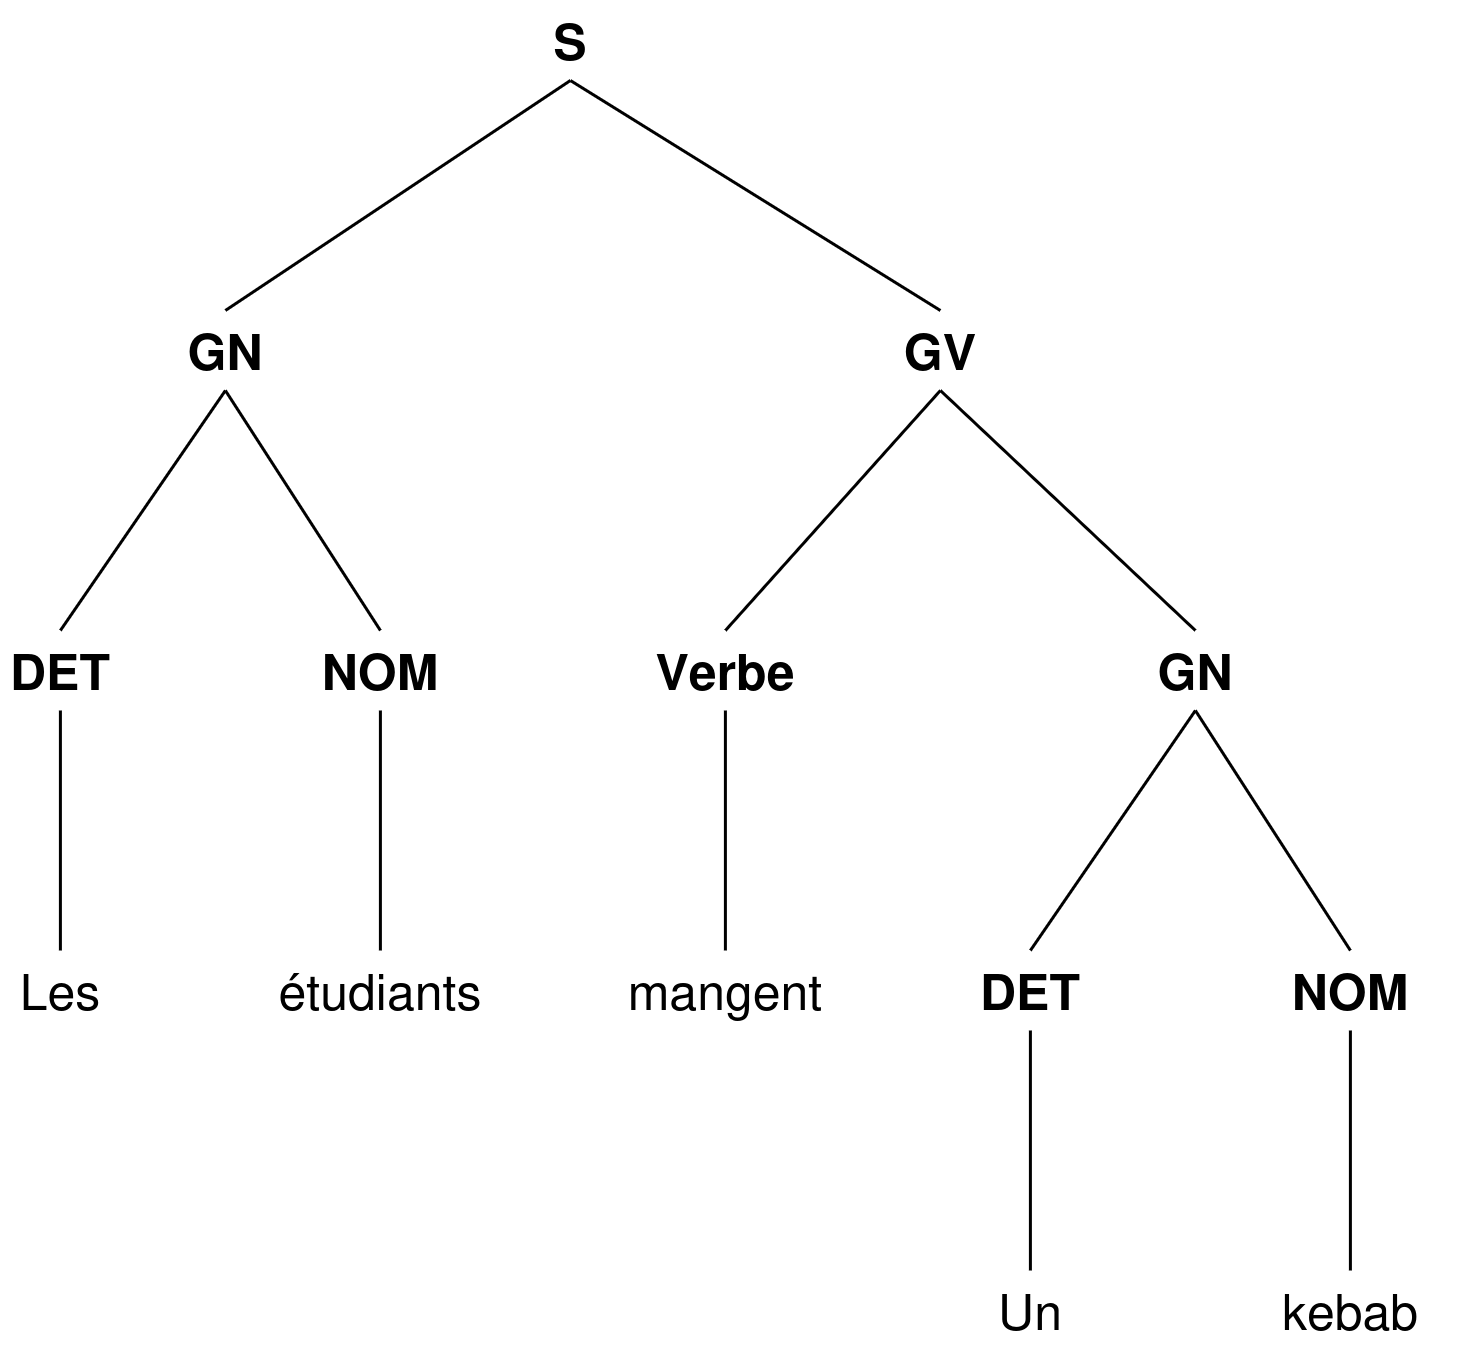
\includegraphics[width=1\columnwidth]{../../../FIGURES/découverte_tal/pos_tagging.png}
        \end{figure}
    \end{minipage}
    \hfill
    \begin{minipage}{0.45\columnwidth}
        \begin{block}{Objectif(s)}
            \begin{itemize}
                \item Associer un mot à sa catégorie
                \item Identifier des structures
                \item Permet de gérer les ambiguïtés
            \end{itemize}
        \end{block}
        \begin{block}{Exemples}
            \begin{itemize}
                \item vers, or, pouvoir, ...
            \end{itemize}
        \end{block}
    \end{minipage}
\end{frame}

\begin{exoframe}{Exercices}
    \begin{block}{Traitez les énoncés suivants}
        \begin{itemize}
            \item 
        \end{itemize}
    \end{block}
\end{exoframe}

\begin{frame}{Limites}
    \begin{block}{Les techniques du TAL sont limitées}
        \begin{itemize}
            \item Des ambiguïtés persistent
            \item Traiter une langue $\ne$ traiter toutes les langues
            \item JAMAIS parfaites (90~\% = environs une faute par phrase)
        \end{itemize}
    \end{block}
\end{frame}


% retour sur difficultés liées au langage

% partie 1 : étude sur divers niveaux linguistiques => phonologie, morphologie, syntaxe, sémantique, pragmatique

% phonologie => phonème, prosodie,variables liées à l'étude du signal => demander à VP martin
% morphologie => morphème, parler de flexions, variantes, préfixe, suffixe, ...
% syntaxe => petit cours de syntaxe et pourquoi c'est utile en TAL
% sémantique => parler de l'alignement morphème / sème et expliquer pk c'est pas parfait + exemples de sens ajoutés, exemples défigements d'expressions
% pragmatique => se renseigner plus

% partie 2 : les outils de base du tal

% lemmatisation
% pos tagging => arbre syntaxique, assigner cat syntaxique
% découpage d'un texte en phrases / section
% identifier sens d'un mot => lexique, dictionnaire, contexte, ...

% fin de la partie 2 : dire que pour certains trucs on a quand même besoin de données sur lesquelles travailler => donner un exemple pour chaque truc ?

% partie 3 : annotation de données
% revoir brièvement les cours de karen là-dessus ou les lui demander

\end{document}
